\documentclass[a4paper,9pt]{extarticle}
\usepackage{kotex}
\usepackage[a4paper,margin=18mm,top=20mm,bottom=20mm]{geometry}
\usepackage{microtype}
\usepackage{tikz}
\usetikzlibrary{arrows.meta,positioning,fit,calc,decorations.pathreplacing}
\usepackage{booktabs,tabularx,array,longtable}
\usepackage{listings}
\usepackage{xcolor}
\usepackage[most]{tcolorbox}
\usepackage{fancyhdr}
\usepackage{titlesec}
\usepackage{hyperref}
\usepackage{enumitem}

\definecolor{navy}{RGB}{0,51,102}
\definecolor{blue}{RGB}{0,102,204}
\definecolor{lightblue}{RGB}{232,242,252}
\definecolor{lightgray}{RGB}{245,246,248}
\definecolor{codegreen}{RGB}{35,120,70}
\hypersetup{colorlinks=true,linkcolor=navy,urlcolor=blue,pdftitle={SWP2P Protocol Manual v1.1.5}}
\pagestyle{fancy}
\fancyhf{}
\lhead{\small\textbf{SWP2P} \quad Protocol Manual}
\rhead{\small Implementation reference \quad v1.1.5}
\cfoot{\thepage}
\renewcommand{\headrulewidth}{0.5pt}
\titleformat{\section}{\large\bfseries\color{navy}}{\thesection}{0.6em}{}[\titlerule]
\titleformat{\subsection}{\normalsize\bfseries\color{navy}}{\thesubsection}{0.6em}{}
\setlist{nosep,leftmargin=1.5em}
\lstset{basicstyle=\ttfamily\small,keywordstyle=\color{blue}\bfseries,commentstyle=\color{codegreen},stringstyle=\color{red!65!black},backgroundcolor=\color{lightgray},frame=single,breaklines=true,showstringspaces=false,columns=fullflexible}

\newcommand{\code}[1]{\texttt{\detokenize{#1}}}
\newcommand{\reg}[1]{\texttt{#1}}
\newcommand{\field}[1]{\textsf{\bfseries #1}}
\newcolumntype{Y}{>{\raggedright\arraybackslash}X}

\begin{document}
\begin{titlepage}
\thispagestyle{empty}
\begin{tikzpicture}[remember picture,overlay]
  \fill[navy] (current page.north west) rectangle ([xshift=12mm]current page.south west);
  \fill[blue] ([xshift=12mm]current page.north west) rectangle ([xshift=15mm]current page.south west);
  \node[anchor=north west,align=left,text width=15cm] at ([xshift=28mm,yshift=-42mm]current page.north west) {
    {\Large\bfseries\color{blue} PROTOCOL MANUAL \& IMPLEMENTATION REFERENCE}\\[5mm]
    {\fontsize{32}{38}\selectfont\bfseries\color{navy} SWP2P}\\[3mm]
    {\Large Open-drain parallel peer-to-peer bus for AVR MCUs}\\[2mm]
    {\large Frame fields, edge cycles, state machine, and source-code mapping}
  };
\end{tikzpicture}
\vspace*{105mm}
\begin{tcolorbox}[colback=lightgray,colframe=navy,title=Document scope]
This manual describes the protocol as implemented by the SWP2P source in this repository. It replaces the earlier v1.0 description where that description differs from the current code. It is an implementation reference, not a claim that every multi-node collision pattern has been hardware-validated.
\end{tcolorbox}
\vspace{8mm}
\begin{tabularx}{\linewidth}{@{}lY@{}}
\textbf{Document version} & v1.1.5 implementation manual \\
\textbf{Target implementation} & Arduino Uno / ATmega328P, AVR registers and interrupts \\
\textbf{Default data width} & W4, preset \code{PRESET_W4_D4_D7} \\
\textbf{Default burst capacity} & \code{SWP2P_MAX_BURST = 16} \\
\textbf{Wire-format change} & DEST(6) + SRC(6) + BURST(1), then LEN or DATA \\
\textbf{License} & See the repository license file \\
\end{tabularx}
\vfill
{\small Sierrastdio \hfill 2026}
\end{titlepage}

\tableofcontents
\clearpage

\section{Purpose and terminology}
SWP2P is a software-defined, multi-node bus. A node can request transmission without a central packet-routing master. One configured node supplies the shared clock; that clock source does not decide which node may transmit. Nodes arbitrate by transmitting the header while BUSY is asserted.

This document distinguishes the \emph{wire protocol} from the \emph{implementation state machine}. Wire fields are the bits visible on DATA lines. State numbers and variable names refer to the current AVR source. Unless stated otherwise, bits are sent most-significant first within each field and each data byte.

\begin{tcolorbox}[colback=lightblue,colframe=blue,title=Important compatibility note]
The v1.1.5 packed header is not wire-compatible with the former two-byte DEST/SRC header. Every node on a shared bus must run a matching implementation. There is no version negotiation or automatic legacy detection.
\end{tcolorbox}

\section{Physical signals and edge convention}
\begin{table}[h]
\centering\small
\caption{Signals used by the Uno implementation}
\begin{tabularx}{\linewidth}{@{}l l l Y@{}}\toprule
Signal & Uno pin & Direction & Implementation meaning \\\midrule
CLK input & D2 / PD2 / INT0 & All nodes receive & Logical-change interrupt. The handler checks the pin level: rising edge is the transmit/update phase; falling edge is the receive/readback phase. \\
CLK output & D9 / PB1 / OC1A & Clock-source node & Timer1 CTC hardware toggles OC1A. Other nodes connect this to D2. \\
BUSY & D3 / PD3 / INT1 & Wired shared line & Active LOW. A transmitter asserts by driving LOW and releases by switching to input/high impedance. \\
ACK & D8 / PB0 & Wired shared line & Active LOW. The addressed receiver asserts ACK after receiving the last data byte; it releases ACK when BUSY returns idle. \\
DATA & Preset dependent & Shared parallel bus & Open-drain style: a node sends 0 by driving LOW and sends 1 by releasing the pin. \\\bottomrule
\end{tabularx}
\end{table}

DATA, BUSY, and ACK use direction-register changes to drive LOW or release the line; external pull-ups establish HIGH. The clock output is generated by the Uno Timer1 OC1A output, not by the DATA open-drain helper. The source configures D2 and D3 for interrupt observation and does not configure the bus pull-ups.

For each wire chunk, the transmitter updates DATA at a rising CLK edge. Receivers sample DATA at the corresponding falling edge. The sender also reads DATA back on falling edges while arbitrating. Consequently, one complete CLK period carries one preset-width chunk, with an update half-cycle and a sample half-cycle.

\section{Frame format}
\subsection{Logical frame}
\begin{center}
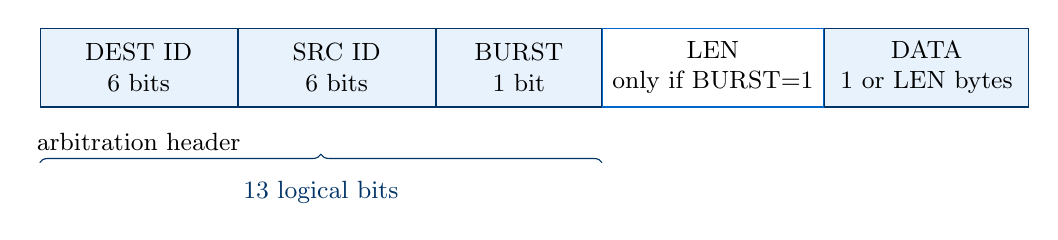
\begin{tikzpicture}[x=1mm,y=1mm,font=\small]
  \tikzset{f/.style={draw=navy,fill=lightblue,minimum height=10mm,align=center,inner sep=2pt}, opt/.style={draw=blue,fill=white,minimum height=10mm,align=center,inner sep=2pt}}
  \node[f,minimum width=25mm] (dest) {DEST ID\\6 bits};
  \node[f,minimum width=25mm,right=0pt of dest] (src) {SRC ID\\6 bits};
  \node[f,minimum width=21mm,right=0pt of src] (burst) {BURST\\1 bit};
  \node[opt,minimum width=28mm,right=0pt of burst] (len) {LEN\\only if BURST=1};
  \node[f,minimum width=26mm,right=0pt of len] (data) {DATA\\1 or LEN bytes};
  \node[below=2mm of dest,align=center] {arbitration header};
  \draw[decorate,decoration={brace,amplitude=3pt},navy] ($(dest.south west)+(0,-7)$) -- ($(burst.south east)+(0,-7)$) node[midway,below=3pt]{13 logical bits};
\end{tikzpicture}
\end{center}

The wire header is the concatenation
\[
  \boxed{\text{DEST}[5:0]}\;\boxed{\text{SRC}[5:0]}\;\boxed{\text{BURST}}.
\]
The header is padded with zero bits at its end to fill an integer number of preset-width chunks. There is no separate start byte: BUSY becoming active starts a frame, and the configured width determines the chunk boundaries.

\begin{table}[h]
\centering\small
\caption{Header fields and encoding}
\begin{tabularx}{\linewidth}{@{}l c Y@{}}\toprule
Field & Width & Meaning \\\midrule
DEST & 6 bits & Destination node ID, 0--62. Value 63 (\code{0x3F}) is reserved for broadcast. \\
SRC & 6 bits & Sender node ID, 0--62. The local constructor masks to six bits and maps local ID 63 to 62. \\
BURST & 1 bit & 0 means one DATA byte follows directly; 1 means LEN then LEN DATA bytes follow. \\
Header padding & 0--7 bits & Trailing zero padding used only to complete the last preset chunk; not a field. \\
LEN & compile-time width & Present only for BURST=1. Encodes \code{len - 2}; bit width depends on \code{SWP2P_MAX_BURST}. \\
DATA & 8 bits per byte & Data is sent MSB first, chunked according to the selected preset width. \\\bottomrule
\end{tabularx}
\end{table}

Broadcast is a destination, not a source identity. A broadcast packet is accepted into the FIFO by every receiver, and every receiver that reaches the ACK state drives the shared ACK line LOW. The sender can observe that the shared ACK line was asserted, but cannot identify which receiver acknowledged.

\subsection{Burst length encoding}
\code{sendBurst()} uses the burst header bit only when \code{len > 1}. For a burst, the transmitted LEN value is \code{len - 2}; the receiver adds 2 after decoding. Thus LEN=0 represents two bytes. LEN width is the minimum width sufficient for the configured maximum and is rounded up to whole DATA chunks.

With the default maximum of 16 bytes, values 0 through 14 are needed, so \code{LEN_BITS=4}. For W4 this is one nibble and there is no LEN padding. The legal wire burst length is 2--16 bytes; a one-byte call through \code{sendBurst()} follows the single-byte path and has BURST=0.

\begin{table}[h]
\centering\small
\caption{Default frame chunk counts (\code{SWP2P_MAX_BURST=16})}
\begin{tabularx}{\linewidth}{@{}c c c c c Y@{}}\toprule
Preset width & Header bits on wire & Header clocks & LEN bits / clocks & Clocks per DATA byte & Notes \\\midrule
W1 & 13 & 13 & 4 / 4 & 8 & Header has no padding. \\
W2 & 14 & 7 & 4 / 2 & 4 & Header has one trailing pad bit. \\
W4 & 16 & 4 & 4 / 1 & 2 & Header has three trailing pad bits. \\
W8 & 16 & 2 & 4 / 1 & 1 & Header has three trailing pad bits. \\\bottomrule
\end{tabularx}
\end{table}

The W4 header still occupies four clocks, just like the former 16-bit header rounded to four nibbles. The compact LEN saves one clock per burst at the default maximum compared with sending an 8-bit LEN over W4 (two clocks). This is a wire-cycle comparison, not a guarantee of a higher safe CLK frequency.

\section{W4 waveform and named cycles}
The following diagrams show the logical W4 bus sequence. Each labeled chunk is one full CLK cycle: the value is driven/updated on CLK rising and sampled on CLK falling. For illustration, the header in the burst diagram is DEST=\code{0x02}, SRC=\code{0x01}, BURST=1. The packed 13 bits plus three pad bits form \code{0x0818}, sent as nibbles \code{0, 8, 1, 8} (bit string \code{0000 1000 0001 1000}).

\begin{figure}[h]
\centering
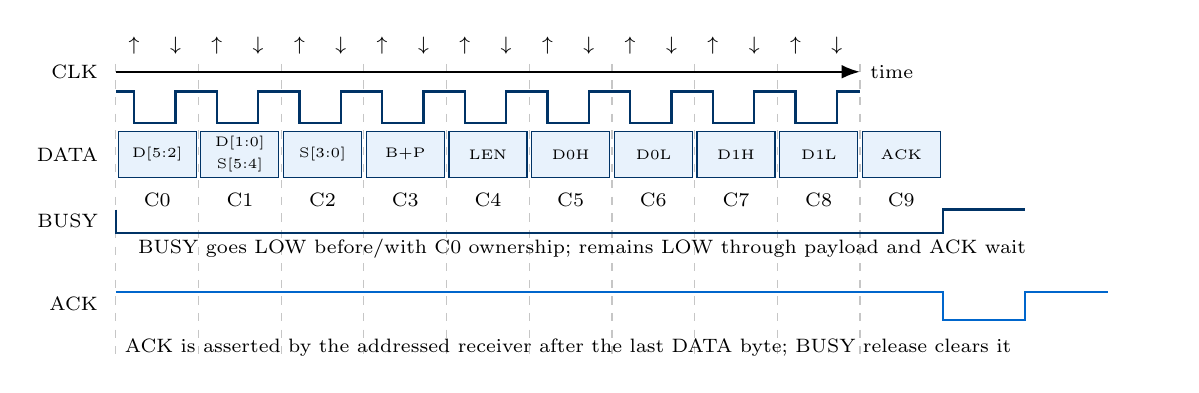
\begin{tikzpicture}[x=1.05cm,y=1cm,font=\scriptsize]
  \def\xstart{2.1}
  \foreach \i/\lab in {0/{D[5:2]},1/{\shortstack{D[1:0]\\S[5:4]}},2/{S[3:0]},3/{B+P},4/{LEN},5/{D0H},6/{D0L},7/{D1H},8/{D1L},9/{ACK}} {
    \pgfmathsetmacro{\x}{\xstart+\i}
    \draw[gray!45,dashed] (\x,0.1) -- (\x,-3.65);
    \node[draw=navy,fill=lightblue,text width=.92cm,minimum width=.92cm,minimum height=.58cm,inner sep=1pt,font=\tiny,align=center] at (\x+.5,-1.05) {\lab};
    \node[below=1mm] at (\x+.5,-1.32) {C\i};
  }
  \draw[-{Latex},thick] (\xstart,0) -- (\xstart+9,0) node[right]{time};
  \node[left] at (2.0,0) {CLK};
  \foreach \i in {0,...,8} {
    \pgfmathsetmacro{\x}{\xstart+\i}
    \draw[navy,thick] (\x,-.25) -- (\x+.22,-.25) -- (\x+.22,-.65) -- (\x+.72,-.65) -- (\x+.72,-.25) -- (\x+1,-.25);
    \node[above=1mm] at (\x+.22,0) {$\uparrow$};
    \node[above=1mm] at (\x+.72,0) {$\downarrow$};
  }
  \node[left] at (2.0,-1.05) {DATA};
  \draw[navy,thick] (2.1,-1.75) -- (2.1,-2.05) -- (12.1,-2.05) -- (12.1,-1.75) -- (13.1,-1.75);
  \node[left] at (2.0,-1.9) {BUSY};
  \node[anchor=west,text width=13cm,align=left] at (2.25,-2.25) {BUSY goes LOW before/with C0 ownership; remains LOW through payload and ACK wait};
  \draw[blue,thick] (2.1,-2.8) -- (12.1,-2.8) -- (12.1,-3.15) -- (13.1,-3.15) -- (13.1,-2.8) -- (14.1,-2.8);
  \node[left] at (2.0,-2.95) {ACK};
  \node[anchor=west,text width=13cm,align=left] at (2.1,-3.5) {ACK is asserted by the addressed receiver after the last DATA byte; BUSY release clears it};
\end{tikzpicture}
\caption{Burst transfer, W4, default 16-byte maximum. C0--C3 are the padded arbitration header; C4 is LEN; each data byte takes two cycles. D=DEST, S=SRC, B=BURST, P=three trailing pad bits; D0H/D0L are the upper/lower nibbles of DATA[0]. The diagram shows two example data bytes, not a fixed frame length.}
\label{fig:w4burst}
\end{figure}

The fourth header nibble is BURST in its most-significant bit followed by three zero pad bits. In C1, the first two bits complete DEST and the remaining two begin SRC. Chunk boundaries do not have to align with field boundaries.

\begin{figure}[h]
\centering\small
\begin{tabularx}{0.96\linewidth}{@{}c Y Y@{}}\toprule
Cycle name & Physical event & State/variable action in the current source \\\midrule
S & BUSY falls; on the next clock rising edge sender asserts BUSY and drives first header chunk C0. & TX: \code{_txState=1} (PENDING) becomes 2 (ARB); \code{_txArbReg}, \code{_arbMyChunk}, \code{_arbChunkCount} initialized. RX starts from INT1 in \code{_onBusyEdge()}. \\
C0...C(A-1) & Header/arbitration chunk. Rising edge updates DATA; falling edge reads it back and receivers accumulate it. & TX compares \code{_arbMyChunk} with \code{_readDataChunk()}; RX accumulates into \code{_rxAddrByte:_rxSrcByte}. \code{A=ADDR_CHUNKS}. \\
L0...L(K-1) & Burst only: LEN chunks. & TX state 3 uses \code{_txDataReg}, \code{_txDataChunkCount}; RX state 3 accumulates \code{_rxDataByte}, then sets \code{_rxLen}. \code{K=LEN_CHUNKS}. \\
D(i,0)... & Data byte i, split into \code{8/DATA_WIDTH} chunks. & TX state 4 advances \code{_txIdx}; RX state 4 assembles \code{_rxDataByte}, then \code{_fifoPush()} stores data and source. \\
ACK & Receiver asserts ACK LOW after its final byte; sender waits a bounded number of CLK edges. & RX state 5 drives PB0/D8. TX state 7 reads ACK and clears \code{FLAG_ACK_FAILED} or sets timeout. \\
IDLE & Sender releases BUSY; line returns HIGH. & INT1 idle path clears busy, releases ACK, resets RX parser; TX clears sending state. \\\bottomrule
\end{tabularx}
\end{figure}

\subsection{Single-byte path}
For a single-byte transfer, BURST=0 and LEN is absent. In W4 the wire chunk order is the four header nibbles, then DATA[7:4], then DATA[3:0], followed by ACK handling. A single byte is fixed-length, so the receiver does not need LEN to find its end.

\subsection{Burst path}
For a burst, BURST=1 and the receiver first reads the configured LEN chunks. After decoding \code{_rxLen = LEN + 2}, it receives exactly that many data bytes, then moves to ACK. There is no per-byte ACK. The FIFO receives each complete byte as it arrives; the application's \code{readBytes()} calls can therefore observe partial FIFO contents while a frame is still arriving.

\section{Arbitration and node filtering}
While multiple senders contend, each sends its header chunks and reads the shared DATA bus back. A sender that detects that it attempted to release a DATA line but observed LOW releases DATA and BUSY, enters TX_LOST, and retries when BUSY returns idle. The receiver side continues parsing the winning header when necessary so a losing node can also receive the winner's packet if addressed to it.

Non-clock-master nodes stop their RX parser once enough header bits identify a non-matching DEST. They do not electrically disconnect: the DATA bus is wired open-drain, and a released line does not interfere with other nodes. The clock-source node continues tracking a non-addressed frame's LEN/data chunk count so it knows when to restore the arbitration clock rate.

\begin{tcolorbox}[colback=lightgray,colframe=navy,title=Implementation limitation]
The code compares multi-bit preset chunks using a bit-mask mismatch test. This is straightforward for W1. For W2/W4/W8 simultaneous collisions, mixed per-line arbitration can produce cases that require a whole-chunk lexicographic comparison to guarantee that exactly one sender wins. This manual records the current implementation; do not treat all simultaneous multi-node arbitration patterns as verified until that behavior is fixed or validated on hardware.
\end{tcolorbox}

\section{Clock generation and dynamic rate}
The node started with \code{begin(true, clkFreq, dataFreq)} generates CLK using Timer1 CTC and OC1A (D9). Other nodes use \code{begin(false)} and follow the external clock on D2. The default base rate is 100 kHz if omitted; the example in the project uses 45 kHz arbitration and 50 kHz payload.

The source calls \code{_clkGoFast()} once the packed header ends and the payload section begins. For a burst, that means the LEN phase and DATA run at \code{dataFreq}; for a single frame DATA runs at \code{dataFreq}. After the final payload, \code{_clkGoSlow()} restores \code{clkFreq} for ACK/idle. Only the clock-source node changes Timer1. Frequency values are not proof of a reliable maximum; ISR execution time and electrical settling still bound practical rates.

\section{Implementation map}
\subsection{State registers}
The state values are stored directly in ATmega328P General Purpose I/O Registers through macros: \code{_txState} is \code{GPIOR1}; \code{_rxState} is \code{GPIOR2}. State transitions occur inside \code{_onClkEdge()} and \code{_onBusyEdge()}.

\begin{table}[h]
\centering\small
\caption{TX and RX states in \code{SWP2P.h}}
\begin{tabularx}{\linewidth}{@{}c l Y c l Y@{}}\toprule
TX & Name & Meaning & RX & Name & Meaning \\\midrule
0 & IDLE & No pending send & 0 & IDLE/FILTERED & No parser work, including filtered non-destination \\
1 & PENDING & Await start/clock edge & 1 & HEADER & Packed DEST/SRC/BURST collection \\
2 & ARB & Send/compare header chunks & 3 & LEN & Receive burst length \\
3 & LEN & Send burst length & 4 & DATA & Receive addressed DATA \\
4 & DATA & Send payload bytes & 5 & ACK & Assert ACK after completed receive \\
6 & LOST & Arbitration lost; retry at idle & 6 & DISCARD & Clock-master counts non-addressed DATA to frame end \\
7 & WAIT\_ACK & Await ACK or timeout & & & \\\bottomrule
\end{tabularx}
\end{table}

\subsection{Frame variables and flags}
\begin{longtable}{@{}p{0.26\linewidth}p{0.17\linewidth}p{0.49\linewidth}@{}}
\caption{Source names mapped to protocol meaning}\label{tab:variables}\\
\toprule Name & Storage & Role \\\midrule\endfirsthead
\toprule Name & Storage & Role \\\midrule\endhead
\code{_nodeId} & static byte & Local source ID, normalized to 0--62 by constructor. \\
\code{_txDestId} & static byte & DEST in low six bits; bit 7 is an internal marker used by \code{sendBurst()}, not a wire header byte. \\
\code{_txLen}, \code{_txIdx} & static bytes & Requested payload length and current TX byte index. \\
\code{_txBuffer[]} / \code{_txData} & static bytes & Copied burst payload / single-byte payload. \code{sendBurst()} copies before returning. \\
\code{_txArbReg} & 16-bit & Left-aligned packed 13-bit header plus trailing preset padding, shifted out MSB-first. \\
\code{_arbChunkCount} & byte & Remaining header chunks after first chunk is driven. \\
\code{_arbMyChunk}, \code{_arbChunksSent} & bytes & Local chunk used for readback arbitration and number of chunks driven. \\
\code{_txDataReg}, \code{_txDataChunkCount} & byte & Shift register and remaining LEN/DATA chunks. \\
\code{_rxAddrByte}, \code{_rxSrcByte} & bytes & Together hold the 16-bit packed-header receive accumulator. After decode, \code{_rxSrcByte} is reused for source ID. \\
\code{_rxDataByte} & byte & LEN accumulator or current DATA byte accumulator. \\
\code{_rxLen}, \code{_rxByteIdx}, \code{_rxChunkCount} & bytes & Decoded data byte count, current byte index, chunks remaining. \\
\code{_rxFifo[]}, \code{_rxSrcFifo[]} & FIFO & Parallel data and sender-ID queues, indexed in lockstep. \\
\code{GPIOR0} flags & register & Sending, busy, addressed-to-me, and ACK-failed flags (bits 0, 1, 3, 5). \\
\code{_ocrArb}, \code{_ocrData} & 16-bit & Timer1 compare values for base and payload rates. \\\bottomrule
\end{longtable}

Header encoding in the TX path is equivalent to
\begin{lstlisting}[language=C++]
header = (DEST << 7) | (SRC << 1) | BURST;
wireHeader = header << (16 - 13); // top-align, then emit preset-width chunks
\end{lstlisting}
The receiver collects the padded wire header and shifts right by \code{ADDR_PADDING_BITS} before extracting DEST, SRC, and BURST.

\section{Application interface and sequence}
\begin{table}[h]
\centering\small
\caption{Common public API}
\begin{tabularx}{\linewidth}{@{}lY@{}}\toprule
API & Behavior \\\midrule
\code{begin(clkIsOutput, clkFreq, dataFreq)} & Initializes pins, interrupts, and optional Timer1 clock output/rates. \\
\code{send(dest, byte)} & Queues one-byte frame (BURST=0); non-blocking. \\
\code{sendBurst(dest, ptr, len)} & Copies data into TX storage and queues a frame; len=1 uses single-byte format. \\
\code{sendBurst(dest, buffer)} & Queues the current \code{SWP2PBuffer} contents. \\
\code{available()} / \code{read()} & Check/read one data byte plus its source ID. \\
\code{readBytes(data, src, max)} & Drains currently available FIFO bytes; it does not wait for whole frame completion. \\
\code{isSending()} / \code{isBusy()} & Report local send-in-progress and shared BUSY status. \\
\code{isAckFailed()} & Returns and clears the most recent ACK-timeout flag. \\\bottomrule
\end{tabularx}
\end{table}

\begin{enumerate}
\item Prepare data in application memory.
\item Call \code{send()} or \code{sendBurst()}. A \code{true} return means accepted into the local TX state machine, not yet delivered.
\item The library arbitrates, sends the frame, and waits for ACK. The application can continue running while the ISR advances the frame.
\item Check \code{isSending()} until it clears, then call \code{isAckFailed()} to inspect the result.
\item On the receiver, drain data and source IDs from the FIFO. A FIFO has depth \code{SWP2P_FIFO_DEPTH} (default 16); it is a byte queue, not a packet queue.
\end{enumerate}

\section{Limits and verification notes}
\begin{itemize}
\item \code{SWP2P_MAX_BURST} is configurable from 1 to 255; it sets the TX storage capacity and compile-time LEN width. The receiver rejects decoded lengths above this configured limit.
\item Node IDs 0--62 are usable; 63 is reserved as broadcast DEST. All nodes on a bus must agree on preset, frame version, maximum burst setting, and compatible clock behavior.
\item There is no CRC/checksum in the frame. ACK confirms that the receiver reached the end of its receive path, not that every data bit was correct.
\item The RX FIFO is byte-oriented and finite (default 16 entries). \code{_fifoPush()} drops a byte silently if the FIFO is full; applications should drain it promptly.
\item The manual's diagrams describe logical edge order. Exact rise/fall time, maximum reliable frequency, and simultaneous arbitration behavior require the actual board, wiring, pull-ups, and source build to validate.
\item On Uno, D9 is Timer1 OC1A and D8 is PB0/ACK in this source. A clock-source node cannot also use a preset that assigns D9 as DATA. D2 and D3 are fixed CLK/BUSY pins. The example's D10 input is separate from W4 D4--D7.
\end{itemize}

\section{Source files}
\begin{itemize}
\item \code{src/SWP2P.h}: public API, TX/RX state machines, ISR handlers, timer-rate transitions.
\item \code{src/SWP2Ppreset.h}: preset pin mappings, open-drain DATA operations, frame-width traits.
\item \code{src/SWP2P.cpp}: static storage, FIFO implementation, Timer1 setup.
\item \code{src/SWP2Pbuffer.h}: application-side fixed-capacity buffer helper.
\end{itemize}

\end{document}
